\section{Programas}\label{sec:programs}

\subsection{Controle da Batelada (PrgBatelada) - SFC}
Este programa implementa a receita de produção utilizando a linguagem \textbf{SFC (Sequential Function Chart)}, ideal para processos em etapas.

A sequência principal consiste em:
\begin{enumerate}
    \item \textbf{Init:} Verifica condições iniciais (Modo Automático, Sem Emergência, TP-01 não cheio).
    \item \textbf{Dosagem:} Abre \texttt{FV101} (Gin) e \texttt{FV102} (Vermouth) sequencialmente até atingir o volume alvo (45L).
    \item \textbf{Mistura e Resfriamento:} Liga o motor \texttt{M101} e abre a refrigeração \texttt{FV103}. Aguarda o nível da jaqueta e a temperatura (TSL101).
    \item \textbf{Transferência:} Drena a jaqueta (\texttt{FV107}) e transfere o produto (\texttt{BA101}, \texttt{FV104}, \texttt{FV105}) para o tanque pulmão.
    \item \textbf{Totalização:} Incrementa os totalizadores globais ao fim do ciclo.
\end{enumerate}

\subsubsection{Rotina de Emergência}
Foi implementada uma "Ilha de Emergência" no SFC. Em caso de acionamento do botão \texttt{EMG} em qualquer etapa crítica, o fluxo é desviado (via \textit{Alternative Branch}) para uma sequência de segurança que:
\begin{itemize}
    \item Fecha todas as admissões imediatamente.
    \item Aguarda 3 segundos.
    \item Configura válvulas de descarte para o Tanque de Rejeitos (\texttt{FV106}).
    \item Esvazia o reator com segurança antes de permitir o rearme.
\end{itemize}

\begin{figure}[H]
    \centering
    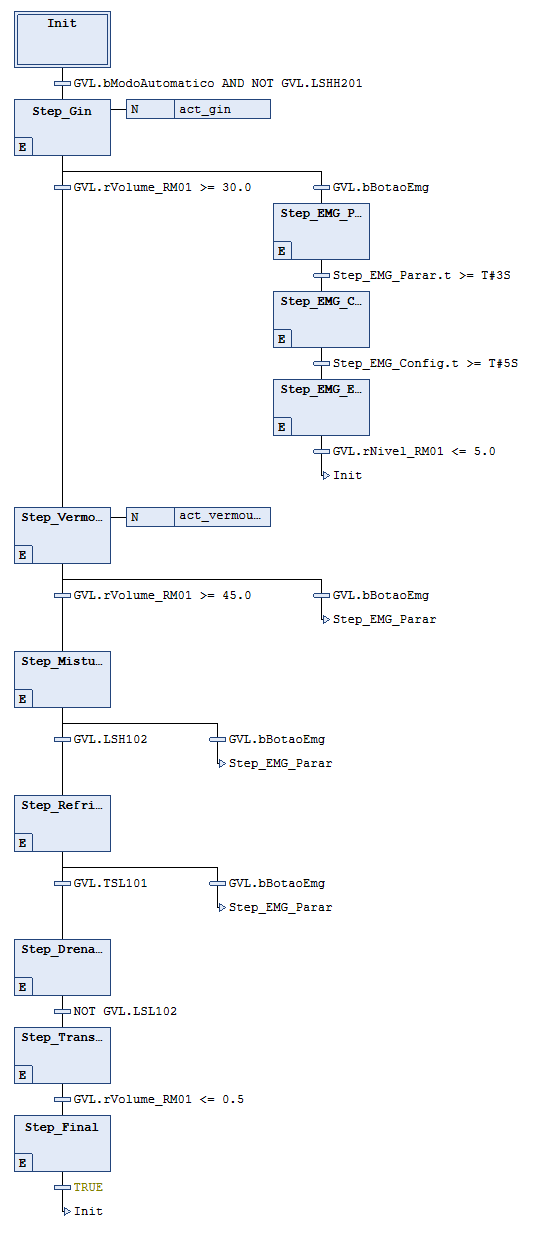
\includegraphics[width=0.6\textwidth]{imgs/SFC-Batelada.png} 
    \caption{Lógica SFC da Batelada com tratamento de Emergência.}
\end{figure}

\subsection{Controle PWM (PrgPWM\_M101) - Texto Estruturado}
Para atender ao requisito de controle de velocidade do misturador com rampas suaves, utilizou-se a linguagem \textbf{ST}.

\textbf{Lógica Implementada:}
\begin{itemize}
    \item \textbf{Rampas:} Dois temporizadores \texttt{TON} controlam a aceleração (0 a 100\% em 5s) e a desaceleração (100 a 0\% em 10s). O cálculo do \textit{Duty Cycle} é feito matematicamente a cada ciclo.
    \item \textbf{Geração de Pulso:} Um timer cíclico de 5ms gera a base de tempo para a frequência de 20Hz. A saída \texttt{xSY101\_PWM\_Out} permanece em nível alto proporcionalmente ao valor da rampa calculado.
\end{itemize}

\begin{lstlisting}
// --- 1. Controle dos Temporizadores ---
// Timer de Subida (5s)
tStartTimer(IN := GVL.bM101_Ligar AND NOT tStopTimer.Q, PT := T#5S);

// Timer de Descida (10s)
tStopTimer(IN := NOT GVL.bM101_Ligar AND NOT tStartTimer.Q, PT := T#10S);

//  2. Calculo da Rampa (0 a 100\%) 
IF tStartTimer.IN OR tStartTimer.Q THEN
    // Converte o tempo decorrido (ET) para Real para fazer a conta
    GVL.rVelocidade_Misturador := (TIME_TO_REAL(tStartTimer.ET) * 100.0) / 5000.0;

ELSIF tStopTimer.IN OR tStopTimer.Q THEN
    // Rampa de descida
    GVL.rVelocidade_Misturador := 100.0 - ((TIME_TO_REAL(tStopTimer.ET) * 100.0) / 10000.0);

ELSIF GVL.bM101_Ligar THEN
    GVL.rVelocidade_Misturador := 100.0;
ELSE
    GVL.rVelocidade_Misturador := 0.0;
END_IF

// Trava de seguranca (Limites)
GVL.rVelocidade_Misturador := LIMIT(0.0, GVL.rVelocidade_Misturador, 100.0);

// --- 3. Geracao do Pulso PWM (20 Hz) ---
tCycleTimer(IN := NOT tCycleTimer.Q, PT := tPeriodo);
IF tCycleTimer.Q THEN
    tCycleTimer(IN := FALSE);
END_IF

// Convertemos tudo para REAL (milissegundos) antes de comparar
GVL.xSY101_PWM_Out := TIME_TO_REAL(tCycleTimer.ET) < (TIME_TO_REAL(tPeriodo) * (GVL.rVelocidade_Misturador / 100.0));
\end{lstlisting}

\subsection{Controle de Envase (PrgArea02\_Envase) - Ladder}
A Área 02 foi desenvolvida em \textbf{Ladder Diagram (LD)} para controle de intertravamentos e lógica contínua.

\textbf{Funcionalidades Principais:}
\begin{itemize}
    \item \textbf{Histerese da Esteira:} A esteira liga apenas se o nível do TP-01 for superior a 50\% e desliga se for inferior a 10\% (utilizando lógica de Set/Reset e comparadores \texttt{GE} e \texttt{LT}).
    \item \textbf{Simulação de Enchimento:} Um bloco \texttt{ADD} incrementa o volume simulado do barril enquanto a válvula \texttt{FV201} está aberta.
    \item \textbf{Contagem:} Um contador \texttt{CTU} registra o número de barris produzidos (\texttt{iContadorBarris}) do tipo WORD.
\end{itemize}

\begin{figure}[H]
    \centering
    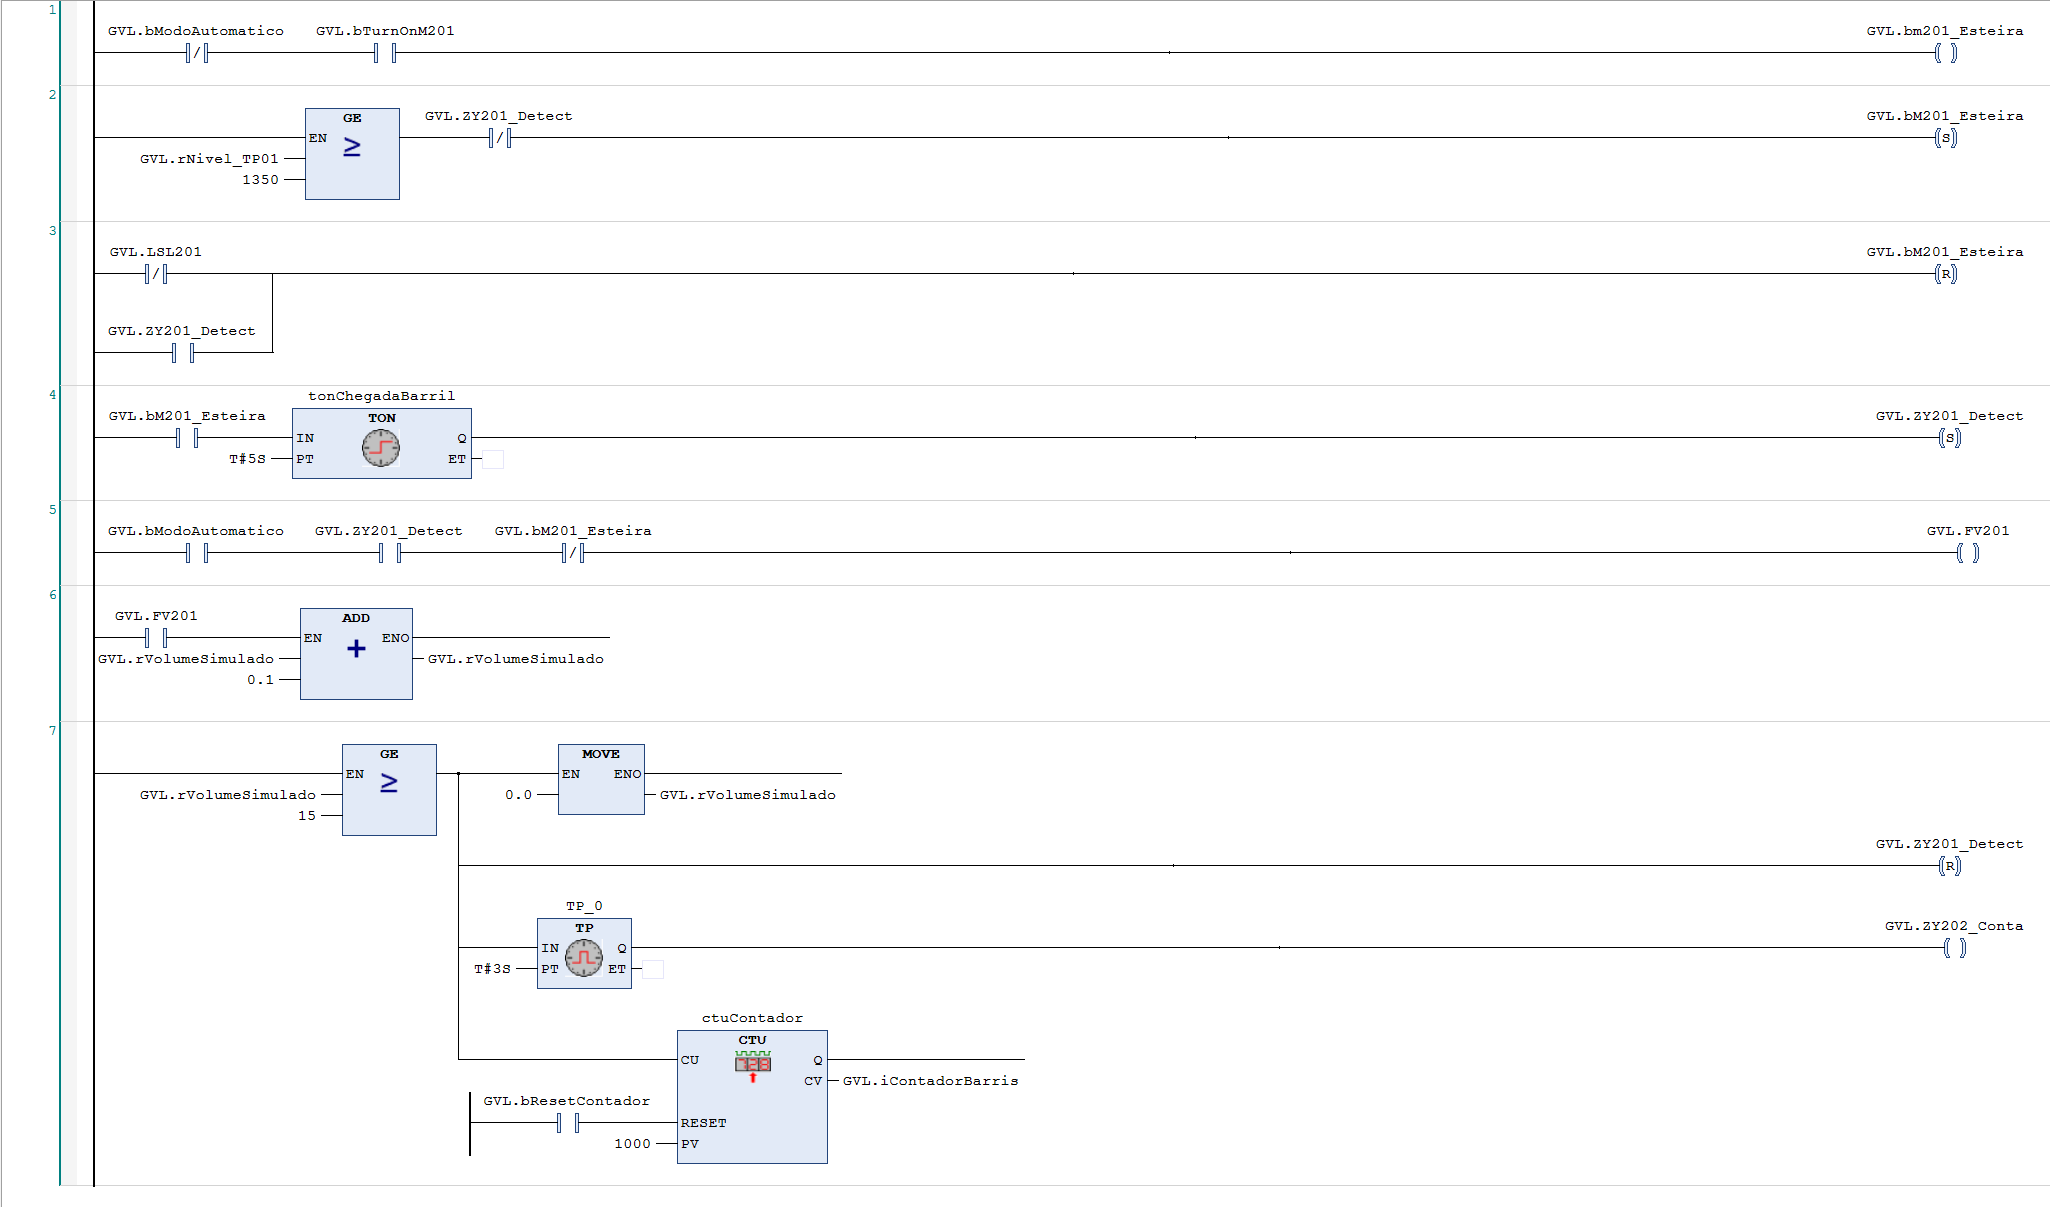
\includegraphics[width=1\textwidth]{imgs/Ladder-Envase.png}
    \caption{Lógica Ladder do controle de envase e esteira.}
\end{figure}

\subsection{Alarmes e Supervisão (PLC\_PRG) - Ladder}
Este programa centraliza a geração de alarmes e a lógica de conversão de sinais analógicos para discretos. Além disso, esse programa é responsável por mudar a variável interna de modo automático, quando o chave de seleção é alterada.
\begin{itemize}
    \item \textbf{Alarmes de Nível:} Comparadores monitoram \texttt{rNivel\_TP01} e acionam flags de alarme para Nível Baixo ($> 10\%$), Alto ($> 85\%$) e Muito Alto ($> 95\%$).
    \item \textbf{Alarme de Transporte:} Um temporizador \texttt{TON} de 15s dispara um alarme se a esteira estiver ligada sem detecção de barris, indicando falha de alimentação.
\end{itemize}


\begin{figure}[H]\label{fig:ladder-prg}
    \centering
    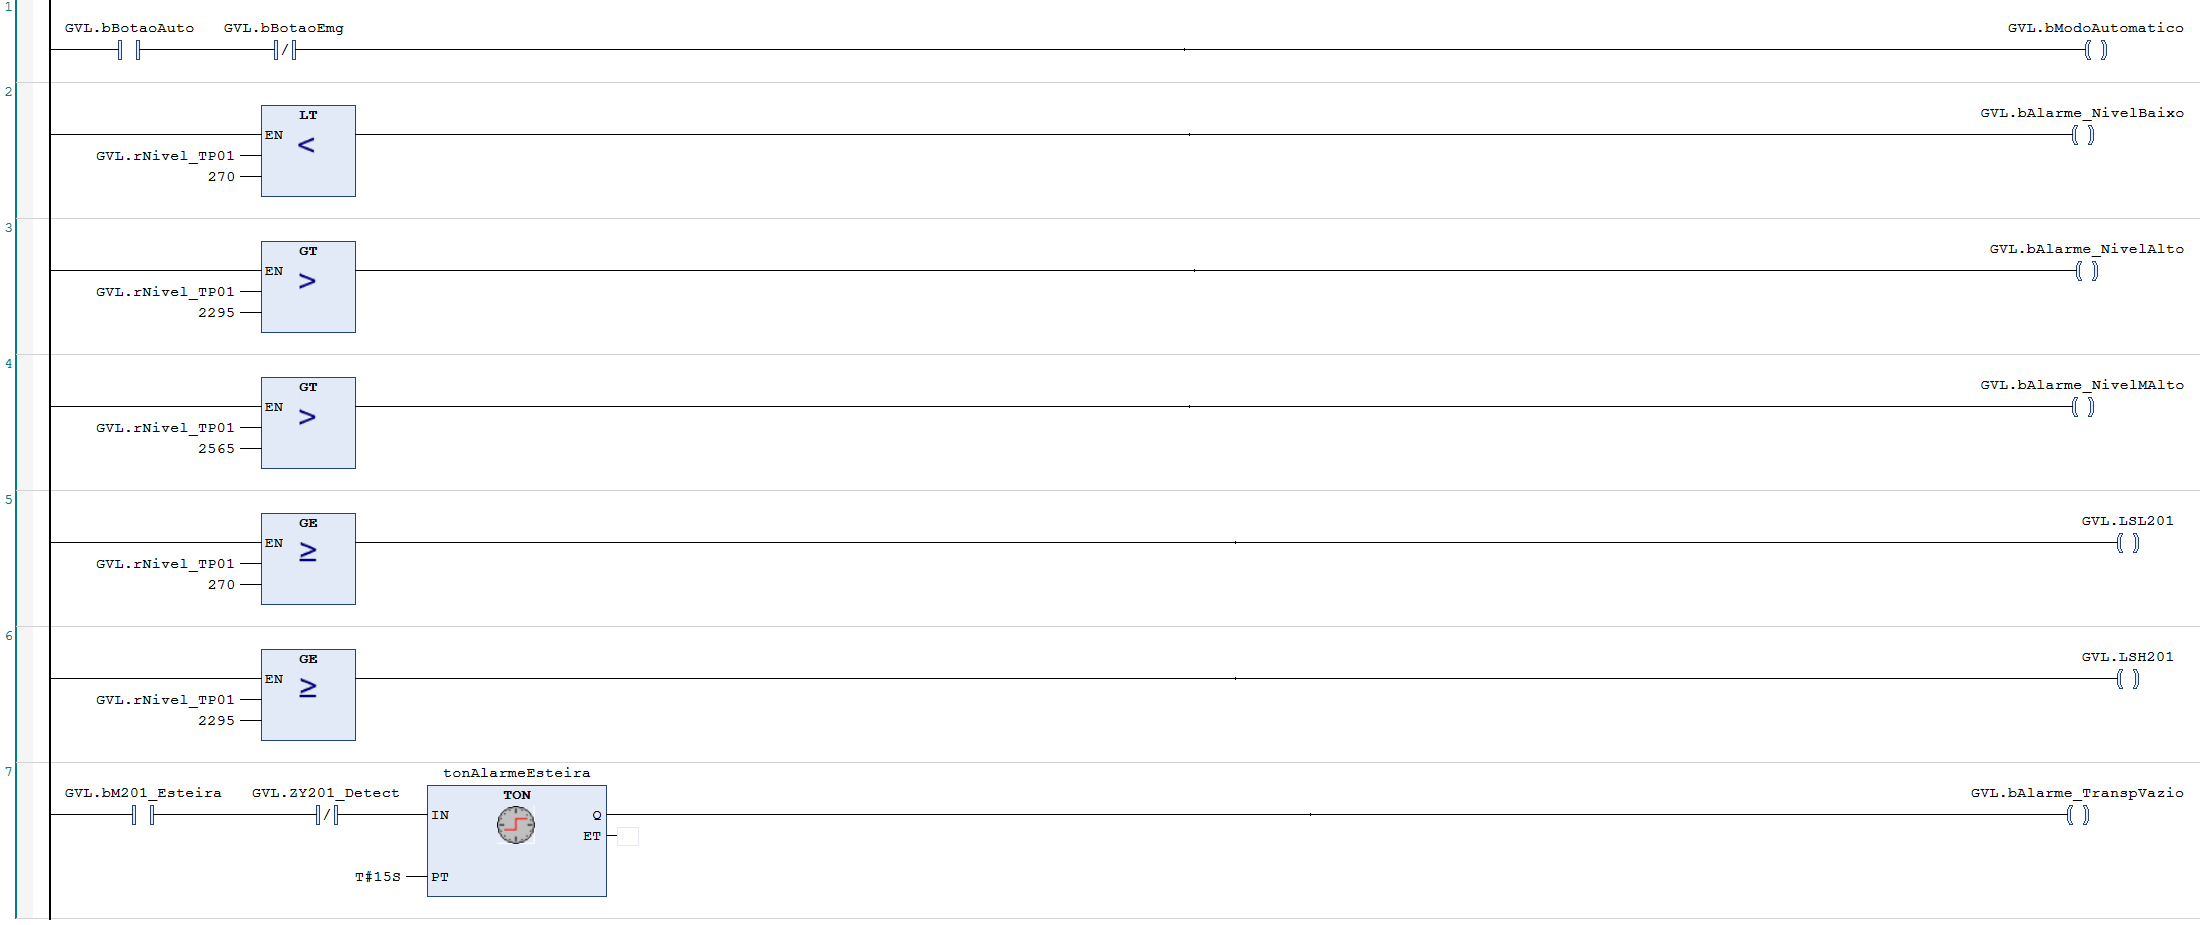
\includegraphics[width=1\textwidth]{imgs/Ladder-Prg.png}
    \caption{Lógica Ladder do controle de alarmes.}
\end{figure}

\subsection{Simulação dos Tanques (Prg\_Simulacao}

Este programa estrutura toda a lógica da planta, modelando desde o comportamento físico dos tanques até o controle automático das operações. Os blocos de tanques calculam nível, temperatura e estados das válvulas; os de dosagem controlam volumes de Gin e Vermouth com precisão; e o de mistura gerencia o motor via PWM com rampas de aceleração e resfriamento da jaqueta térmica. A transferência para o tanque pulmão é regulada por histerese de nível, enquanto a área de envase utiliza blocos para sincronizar sensores, esteira transportadora e a válvula de enchimento. Complementando o sistema, blocos de alarmes e segurança monitoram falhas (como ausência de barris), níveis críticos e condições de emergência, garantindo parada segura e intertravamentos adequados. Em conjunto, esses blocs modularizam o processo e permitem uma simulação realista e organizada conforme a IEC 61131-3.

\begin{figure}[H]\label{fig:ladder-simu}
    \centering
    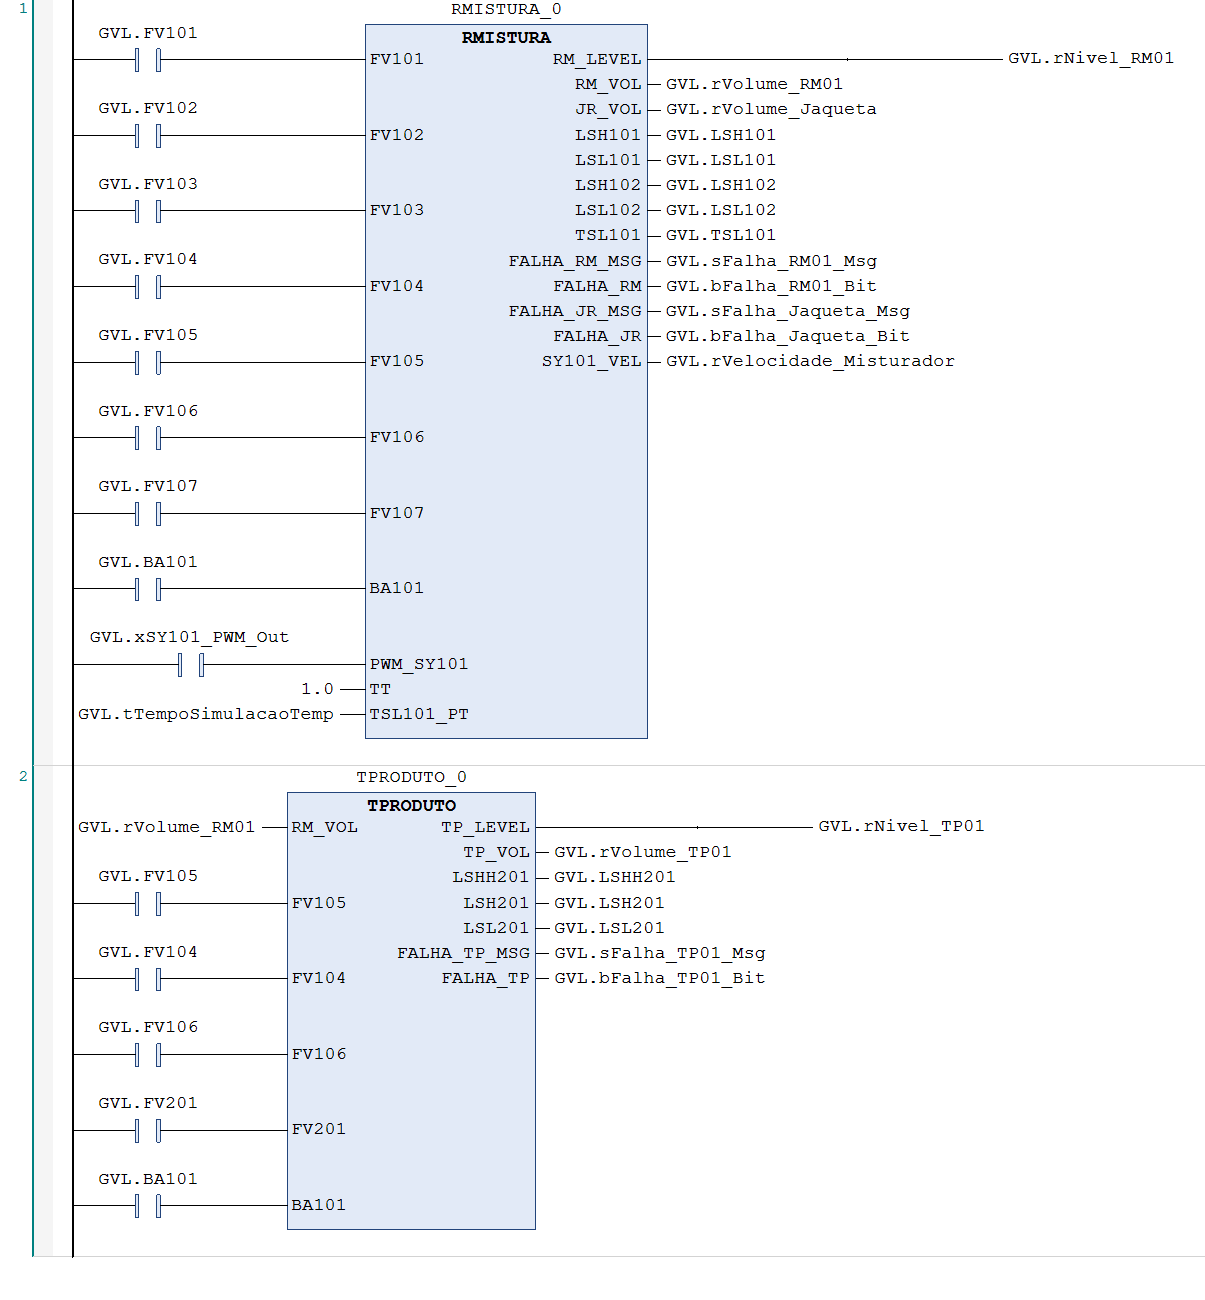
\includegraphics[width=1\textwidth]{imgs/Ladder_Simulacao.png}
    \caption{Lógica Ladder do controle dos Tanques.}
\end{figure}